\chapter{Practice Exam 4}
    Anna the Audiophile has asked for your help to build an amplifier and filter to take small
    signals from her hifi system and amplify them so that she can drive her new subwoofer. The
    hifi system produces AC signals at varying frequencies with 250 mVrms maximum magnitude.
    Her subwoofer requires the signals to be 20 Vrms maximum magnitude. The signals that Anna
    is interested in are below 200 Hz. She would like the filter to attenuate signals at frequencies
    above 200 Hz.
    \begin{figure}[H]
        \centering
        \includegraphics[width=0.6\linewidth]{figures/exams/audiophile.png}
    \end{figure}
    \begin{enumerate}
        \item Design the amplifier and filter circuit to meet Anna’s requirements. The circuit must
        produce the required gain, and also attenuate the signals above 200 Hz. Show
        calculations for the selection of components where practical. Show a circuit diagram for
        the complete amplifier and filter circuit\\
            \textbf{Solution:}\\
            The filter must attenuate all frequencies above 200 Hz. And must increase the gain of the
            input signal. Therefore, an active low-pass filter was chosen.\\
            As it needs to amplify signals from 250 mVrms to 20 Vrms, the gain of the amplifier must be 80.\\
            \begin{minipage}{0.6\linewidth}
                \begin{figure}[H]
                    \centering
                    \begin{circuitikz}[american]
                        \draw (0,0) node[op amp] (opamp) {};
                        \node[above left] at (-3,0.7) {250mV RMS};
                        \draw (-3.5,0.5) to[resistor, R=1k$\Omega$] (opamp.-);
                        \draw (opamp.-) to[short] ++(0,1) to[resistor, R=80k$\Omega$]++(3,0) to[short] ++(0,-1.5);
                        \draw (opamp.-) to[short] ++(0,2.5) to[capacitor, C=10nF] ++(3,0) to[short] ++(0,-3);
                        \draw (opamp.out) to[short] ++(2,0) node[above] {20V RMS};
                        % ground
                        \draw (opamp.+) to[short] ++(-0.5,0) to[short] ++(0,-0.5) node[ground] {};
                    \end{circuitikz}
                \end{figure}
            \end{minipage}
            \begin{minipage}{0.3\linewidth}
                \begin{flalign*}
                    \left|\text{Gain}\right| = \left|-\frac{R_2}{R_1}\right| &= 80\\
                    \text{Let } R_1 &= 1k\Omega\\
                    \therefore R_2 &= 80k\Omega\\
                    C &= \frac{1}{2\pi f R_2}\\
                    &= \frac{1}{2\pi \times 200\times 80\times 10^3}\\
                    &= 10\text{nF}
                \end{flalign*}
            \end{minipage}
        \item Anna reads the subwoofer manual and notes the value of DC blocking capacitor
        C1 = 1000 $\mu$F. She wonders how the capacitor will affect the frequency response of the
        subwoofer. What kind of filter is formed by C1 and the speaker resistance? Calculate the
        cut-off frequency of this filter. Describe the behaviour of this filter in words.\\
            \textbf{Solution:}\\
            The capacitor and the speaker resistance form a high-pass filter with a cut-off frequency 
            defined by
            \begin{align*}
                f_c &= \frac{1}{2\pi R C}\\
                &= \frac{1}{4\times 1000\times 10^{-6}\times 2\pi}\\
                &= 40\text{Hz}
            \end{align*}
            This filter will attenuate all frequencies below 40 Hz.
        \item When first turned on, Anna’s amplifier fails and applies +15V DC directly to the output
        (va). After 30 milliseconds, the speaker protection circuit operates Sw1 to disconnect the
        speaker and connect it to ground (Sw1 changes from position ‘1’ to position ‘2’). Taking
        the time the amplifier was turned on as t=0 seconds, calculate and plot the voltage across
        the speaker for the first 60 milliseconds. Ensure your drawing is to scale and has labelled
        key values\\
            \textbf{Solution:}\\
            First isolate the circuit at $t=0$.\\
            \begin{minipage}{0.6\linewidth}
                \begin{figure}[H]
                    \centering
                    \begin{circuitikz}[american]
                        \draw (0,0) 
                            to[voltage source, invert, v=15V] (0,2)
                            to[capacitor, l=100$\mu F$] (2,2)
                            to[resistor, R=4$\Omega$] (2,0)
                            to[short] (0,0); 
                    \end{circuitikz}
                \end{figure}
                Apply source transformation from Thevenin to Norton equivalent\\($I = \frac{V}{R} = \frac{15}{4} = 3.75A$)
                \begin{figure}[H]
                    \centering
                    \begin{circuitikz}[american]
                        \draw (0,0)
                            to[current source, i=3.75A] (0,2)
                            to[short] (4,2)
                            to[capacitor, l=100$\mu$F] (4,0)
                            to[short] (0,0);
                        \draw (2,0) to[resistor, R=4$\Omega$] (2,2);
                    \end{circuitikz}
                \end{figure}
                \begin{figure}[H]
                    \centering
                    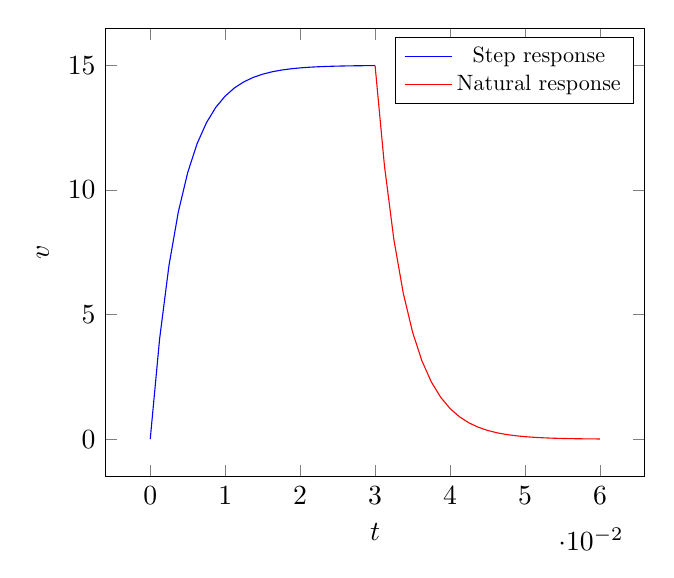
\begin{tikzpicture}
                        \begin{axis}[
                            xlabel=$t$,
                            ylabel=$v$,
                            legend style={nodes={scale=0.8, transform shape}},
                        ]
                        \addplot[blue, domain=0:0.03] {15 - 15*exp(-250*x)};
                        \addplot[red, domain=0.03:0.06] {14.9917*exp(-250*(x-0.03))};
                        \legend{Step response, Natural response}
                        \end{axis}
                    \end{tikzpicture}
                    \caption{Voltage across the speaker}
                \end{figure}
            \end{minipage}
            \begin{minipage}{0.4\linewidth}
                For step response ($0<t<0.03$) (capacitor charging)
                \begin{flalign*}
                    v(t) &= I_s R + (V_o - I_s R)e^{-\frac{t}{RC}}\\
                    &= 3.75\times 4 + (0 - 3.75\times 4)e^{-\frac{t}{100\times 10^{-6}\times 4}}\\
                    &= 15 - 15e^{-250t}\\
                    v(0.03) &= 15 - 15e^{-250\times 0.03} = 14.9917\\
                    \intertext{For natural response ($t>0.03$) (capacitor discharging), $V_o = 14.9917$}
                    v(t) &= V_o e^{-\frac{t-0.03}{RC}}\\
                    &= 14.9917e^{-250(t-0.03)}\\\\\\\\\\\\\\\\\\\\\\\\\\\\\\
                \end{flalign*}
            \end{minipage}\\
        \item The amplifier fault has now been fixed and the system works normally (Sw1 is in
        position ‘1’). Perform frequency response analysis for the amplifier and filter you
        designed in part (a) to calculate the gain in dB and phase in degrees when the hifi system
        sends a signal at 10 Hz, 100 Hz and 1000 Hz.\\
            \textbf{Solution:}\\
            \begin{flalign*}
                H(\omega) &= -\frac{R_2}{R_1} \frac{\frac{1}{R_2 C}}{j\omega + \frac{1}{R_2 C}} \tag{$\frac{1}{R_2C} = \frac{1}{80\times 10^{3}\times10^{-9}} = 1250$}\\
                &= -80\frac{1250}{j\omega + 1250}
            \end{flalign*}
            \begin{figure}[H]
                \centering
                \begin{tabular}{cccc}
                    $\boldsymbol{\omega}$ & $\textbf{H}(\boldsymbol{\omega})$ & $\textbf{Gain (dB)}$ & $\textbf{Phase (degrees)}$\\
                    \toprule
                    $20\pi$ & $79.899\angle 177.122^{\circ}$ & 38.051 & 177.122\\
                    $200\pi$ & $71.4781\angle 153.313^{\circ}$ & 37.084 & 153.313\\
                    $2000\pi$ & $15.6096\angle 101.252^{\circ}$ & 23.868 & 101.252\\
                    \bottomrule
                \end{tabular}
                \caption{Frequency response analysis}
            \end{figure}
        \item Calculate the output voltage of the amplifier and filter circuit (va) when a 250 mVrms,
        100 Hz signal is applied at its input ($v_{in}$)\\
            \textbf{Solution:}
            \begin{flalign*}
                V_{out} &= V_{in}H(\omega)\\
                &= 0.25\times\sqrt{2} \times H(200\pi)\\
                &= 0.25\times\sqrt{2} \times 71.4781\angle 153.313^{\circ} \tag{From part (d)}\\
                &= 25.2713\angle 153.313^{\circ}
            \end{flalign*}
    \end{enumerate}